
%%%%%%%%%%%%%%%%%%%%%%%%%%%%%%%%%%%%%%%%%
% Focus Beamer Presentation
% LaTeX Template
% Version 1.0 (8/8/18)
%
% This template has been downloaded from:
% http://www.LaTeXTemplates.com
%
% Original author:
% Pasquale Africa (https://github.com/elauksap/focus-beamertheme) with modifications by 
% Vel (vel@LaTeXTemplates.com)
%
% Template license:
% GNU GPL v3.0 License
%
% Important note:
% The bibliography/references need to be compiled with bibtex.
%
%%%%%%%%%%%%%%%%%%%%%%%%%%%%%%%%%%%%%%%%%

%----------------------------------------------------------------------------------------
%	PACKAGES AND OTHER DOCUMENT CONFIGURATIONS
%----------------------------------------------------------------------------------------

\documentclass{beamer}
% \usepackage{enumitem}
\beamertemplatenavigationsymbolsempty % suppress navigation bar

\usetheme{default} % Use the Focus theme supplied with the template
% Add option [numbering=none] to disable the footer progress bar
% Add option [numbering=fullbar] to show the footer progress bar as always full with a slide count

% Uncomment to enable the ice-blue theme
%\definecolor{main}{RGB}{92, 138, 168}
%\definecolor{background}{RGB}{240, 247, 255}

%------------------------------------------------

\usepackage{booktabs} % Required for better table rules

\begin{document}

\begin{frame}{Trash Mergers}
\centering

\includegraphics[width = \textwidth]{images/wmiannounce.png}
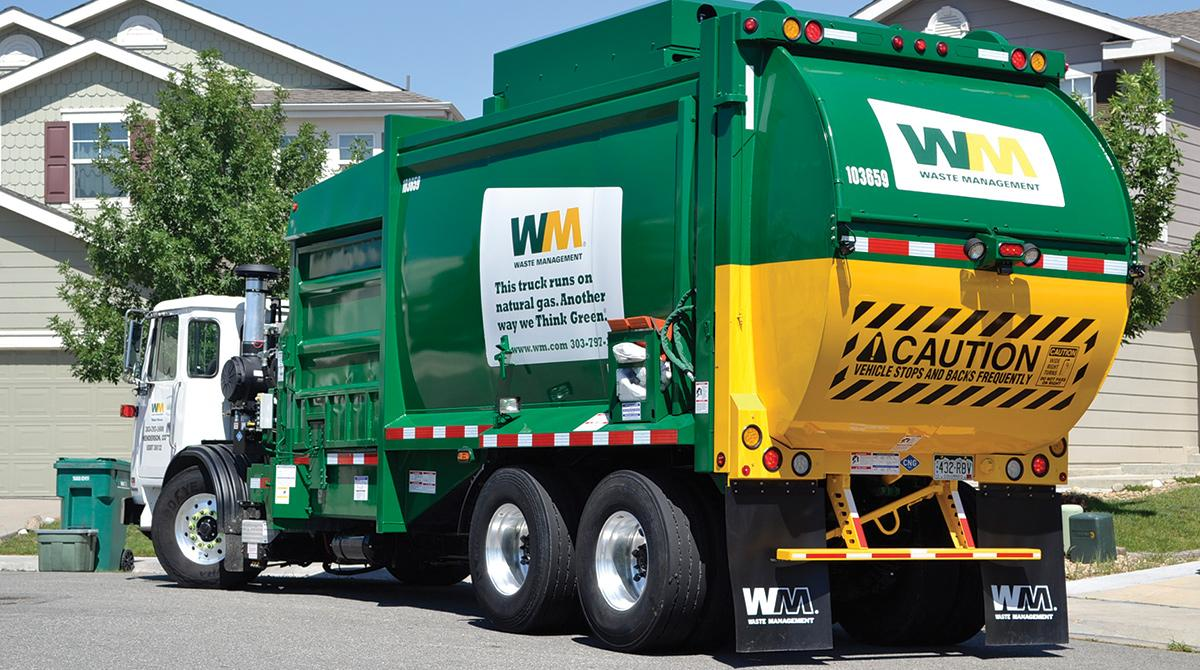
\includegraphics[width = \textwidth, height = .55\textheight]{images/wmtruck.png}
\end{frame}

\begin{frame}{Market Shares (2019)}
\begin{table}
\centering
 \begin{tabular}{r l c c}
Rank & Firm & Revenue (\$ millions) & Share (\%) \\ %[0.5ex] 
 \hline\hline
1 & Waste Management & 15,455 & 46.1 \\
2 & Republic Services & 10,299 &  30.1\\
3 & Waste Connections & 5,388 & 16.1\\
4 & Advanced Disposal & 1,623 & 4.8 \\
5 & Casella Waste & 743 & 2.2\\ \hline \hline 
& Total & 33,508 & 100
 \end{tabular}
\caption{Operating  revenues in North America as reported by Statista for 2019. Smaller competitors are excluded from these calculations.}
\end{table}
\end{frame}

\begin{frame}{Waste Management (WM) Facilities}
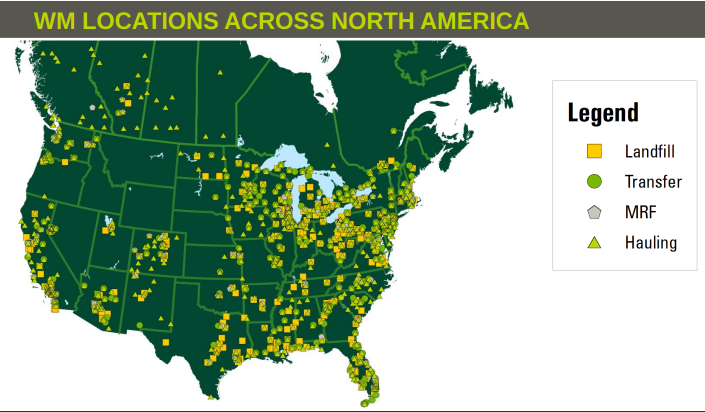
\includegraphics[width = \textwidth]{images/wmlocations.png}
\end{frame}

\begin{frame}{Advanced Disposal (ADS) Facilities}
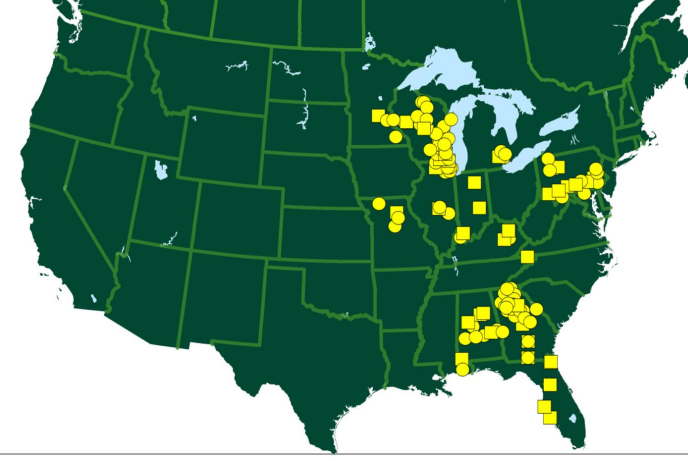
\includegraphics[width = \textwidth]{images/adslocations.png}
\end{frame}

\begin{frame}{Deal Rationale}
Why does WM want to buy ADS?
\begin{itemize}
\item Expects ``more than \$100M in potential annual cost and capital expenditure synergies" (i.e., lower \textbf{fixed costs}!)
\item Capture \textbf{economies of scale} by serving more customers
\item Acquire \textbf{market power} by reducing competition
\end{itemize}
\end{frame}

\begin{frame}{Antitrust concern: control over indispensable inputs}
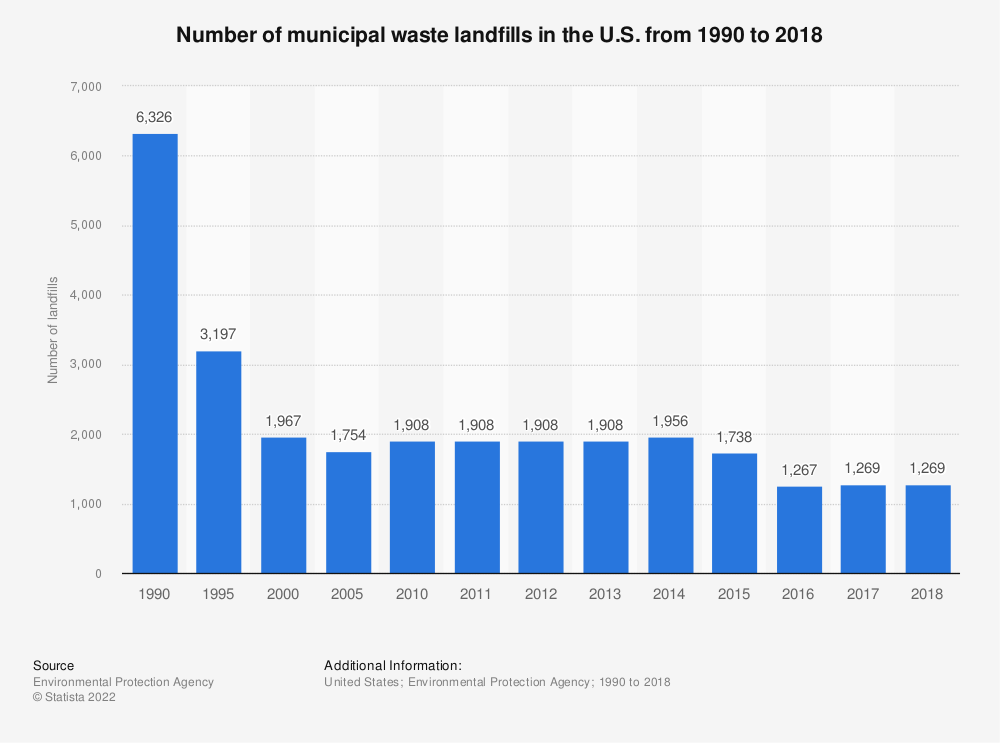
\includegraphics[width = \textwidth]{images/landfills.png}
\end{frame}

\begin{frame}{Antitrust concern: economies of scale}
Once WM routes a garbage truck down the street, it doesn't cost very much to stop at one more house. \vspace{1em}


\includegraphics[width = \textwidth]{images/streethouses.jpg}
\vspace{.1em}

In other words, adding another customer to the route \textbf{lowers} the \textbf{average cost}!
\end{frame}

\begin{frame}{Antitrust solution: divestitures (aka, the DOJ strikes back)} 

WM must sell some of their assets to a 3rd party (GFL Environmental)
\begin{itemize}
\item 15 landfills
\item 37 transfer stations
\item 29 hauling locations
\item over 200 waste collection routes
\end{itemize}
\vspace{2em}

This will ``ensure that businesses, municipalities, and towns continue to benefit from \textbf{competition} for these critical services."
\end{frame}

\end{document}
